\documentclass[crop,border={2pt 2pt 2pt 2pt},tikz]{standalone}
\usepackage{braket}
\usepackage{bbold}
\usepackage{bm}
\usepackage{amsmath}



\usetikzlibrary{backgrounds,decorations.markings}
\tikzset{>=latex}
\tikzset{->-/.style={decoration={
  markings,
  mark=at position .5 with {\arrow{>}}},postaction={decorate}}}
\begin{document}
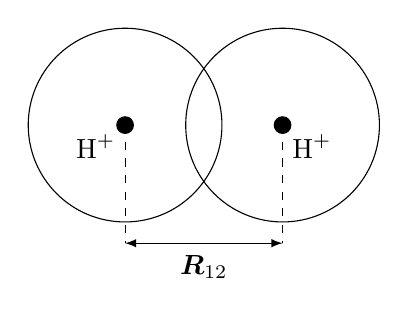
\begin{tikzpicture}
    \draw[black, fill] (0,0) circle (3pt) node[anchor= north east] {$\text{H}^+$};
    \draw[black] (0,0) circle (35pt);

    \draw[black, fill] (2,0) circle (3pt) node[anchor=north west] {$\text{H}^+$};
    \draw[black] (2,0) circle (35pt);
    \draw[black, dashed] (0,0) -- (0,-1.5);
    \draw[black, dashed] (2,0) -- (2,-1.5);
    \draw[<->] (0,-1.5) -- (2, -1.5); 
    \node at (1, -1.8) {$\bm R_{12}$};

\end{tikzpicture}
\end{document}
 
